%package list
\documentclass{article}
\usepackage[top=3cm, bottom=3cm, outer=3cm, inner=3cm]{geometry}
\usepackage{graphicx}
\usepackage{url}
%\usepackage{cite}
\usepackage{hyperref}
\usepackage{array}
%\usepackage{multicol}
\newcolumntype{x}[1]{>{\centering\arraybackslash\hspace{0pt}}p{#1}}
\usepackage{natbib}
\usepackage{pdfpages}
\usepackage{multirow}
\usepackage{multirow}
\usepackage[normalem]{ulem}
\useunder{\uline}{\ul}{}
\usepackage{amsmath}
\usepackage{float}
\usepackage{multicol}
\usepackage{subcaption}


% para tener url cortas en bib
\let\oldUrl\url
\renewcommand{\url}[1]{\href{#1}{Enlace}}
%

%%%%%%%%%%%%%%%%%%%%%%%%%%%%%%%%%%%%%%%%%%%%%%%%%%%%%%%%%%%%%%%%%%%%%%%%%%%%
%%%%%%%%%%%%%%%%%%%%%%%%%%%%%%%%%%%%%%%%%%%%%%%%%%%%%%%%%%%%%%%%%%%%%%%%%%%%
\newcommand{\csemail}{vmachacaa@ulasalle.edu.pe}
%\newcommand{\csdocente}{MSc. Vicente Enrique Machaca Arceda}
\newcommand{\csdocente}{Enzo Velásquez Lobatón \\
	Carlo Corrales Delgado\\
	Oscar Ramirez Valdez\\
	Vicente Machaca Arceda}
\newcommand{\cscurso}{Computación de Alto Desempeño}
\newcommand{\csuniversidad}{Universidad Nacional de San Agustín de Arequipa}
\newcommand{\csescuela}{Doctorado en Ciencias de la Computación}
\newcommand{\cspracnr}{03}
\newcommand{\cstema}{Centro de datos de Telefónica}
%%%%%%%%%%%%%%%%%%%%%%%%%%%%%%%%%%%%%%%%%%%%%%%%%%%%%%%%%%%%%%%%%%%%%%%%%%%%
%%%%%%%%%%%%%%%%%%%%%%%%%%%%%%%%%%%%%%%%%%%%%%%%%%%%%%%%%%%%%%%%%%%%%%%%%%%%


\usepackage[english,spanish]{babel}
\usepackage[utf8]{inputenc}
\AtBeginDocument{\selectlanguage{spanish}}
\renewcommand{\figurename}{Figura}
\renewcommand{\refname}{Referencias}
\renewcommand{\tablename}{Tabla} %esto no funciona cuando se usa babel
\AtBeginDocument{%
	\renewcommand\tablename{Tabla}
}

\usepackage{fancyhdr}
\pagestyle{fancy}
\fancyhf{}
\setlength{\headheight}{30pt}
\renewcommand{\headrulewidth}{1pt}
\renewcommand{\footrulewidth}{1pt}
\fancyhead[L]{\raisebox{-0.2\height}{
\includegraphics[width=3cm]{img/logo_unsa}}}
\fancyhead[C]{}
\fancyhead[R]{\fontsize{7}{7}\selectfont	\csuniversidad \\ \csescuela \\ \textbf{\cscurso} }
\fancyfoot[L]{Vicente, Enzo, Oscar y Carlos}
\fancyfoot[C]{\cscurso}
\fancyfoot[R]{Página \thepage}


% para el codigo fuente
\usepackage{listings}
\usepackage{color}
\definecolor{dkgreen}{rgb}{0,0.6,0}
\definecolor{gray}{rgb}{0.5,0.5,0.5}
\definecolor{mauve}{rgb}{0.58,0,0.82}
\lstset{frame=tb,
	language=Python,
	aboveskip=3mm,
	belowskip=3mm,
	showstringspaces=false,
	columns=flexible,
	basicstyle={\small\ttfamily},
	numbers=none,
	numberstyle=\tiny\color{gray},
	keywordstyle=\color{blue},
	commentstyle=\color{dkgreen},
	stringstyle=\color{mauve},
	breaklines=true,
	breakatwhitespace=true,
	tabsize=3
}




\begin{document}
	
	
	
	
\begin{titlepage}
	
	\newcommand{\HRule}{\rule{\linewidth}{0.5mm}} % Defines a new command for the horizontal lines, change thickness here
	
	\center % Center everything on the page
	
	%----------------------------------------------------------------------------------------
	%	HEADING SECTIONS
	%----------------------------------------------------------------------------------------
	
	\textsc{\LARGE \csuniversidad}\\[1.5cm] % Name of your university/college
	\textsc{\Large \cscurso}\\[0.5cm] % Major heading such as course name
	%\textsc{\large Assignment 1}\\[0.5cm] % Minor heading such as course title
	
	%----------------------------------------------------------------------------------------
	%	TITLE SECTION
	%----------------------------------------------------------------------------------------
	
	\vspace{2cm}
	
	\HRule \\[0.4cm]
	{ \huge \bfseries \cstema}\\[0.4cm] % Title of your document
	\HRule \\[1.5cm]
	
	%----------------------------------------------------------------------------------------
	%	AUTHOR SECTION
	%----------------------------------------------------------------------------------------
	
	\begin{minipage}{0.4\textwidth}
		\begin{flushleft} \large
			\emph{Alumnos:}\\
			\csdocente
		\end{flushleft}
	\end{minipage}
	~
	\begin{minipage}{0.4\textwidth}
		\begin{flushright} \large
			\emph{Docente:} \\
			PhD. Alvaro Mamani Aliaga
		\end{flushright}
	\end{minipage}\\[2cm]
	
	% If you don't want a supervisor, uncomment the two lines below and remove the section above
	%\Large \emph{Author:}\\
	%John \textsc{Smith}\\[3cm] % Your name
	
	%----------------------------------------------------------------------------------------
	%	DATE SECTION
	%----------------------------------------------------------------------------------------
	
	{\large \today}\\[2cm] % Date, change the \today to a set date if you want to be precise
	
	%----------------------------------------------------------------------------------------
	%	LOGO SECTION
	%----------------------------------------------------------------------------------------
	
	
\includegraphics[width=100px, keepaspectratio]{img/unsa}\\[1cm] % Include a department/university logo - this will require the graphicx package
	
	%----------------------------------------------------------------------------------------
	
	\vfill % Fill the rest of the page with whitespace
	
\end{titlepage}	
	
	
	

	
	
\tableofcontents
\newpage	
	

	
		
	
\section{Introducción}
	
En la actualidad estamos viviendo la era de la información, la cantidad de datos crecen exponencialmente y esto conlleva a incrementar los requerimientos de espacio y un alto consumo de  energia \citep{baliga2010green, kant2009data}. Además, a pesar de todas la ventajas de la computación de la nube y las nuevas oportunidades que genera, cada vez son mas las grandes compañias que ven sus recursos agotados, en este contexto es mas eficiente tener cientos de servidores en comparación que un solo servidor de gran capacidad \citep{chandransurvey}. Si a esto adicionamos el aumento en uso de las redes 4G y 5G y la cantidad de información que generan, estos van a representar nuevos retos a solucionar en un temprano a mediano plazo.\\
	
Toda la información mencionada anteriormente necesita estar alojada  y administrada en los centros de datos. Estos son instalaciones de  gran tamaño con numeros equipos como servidores, sistemas de refrigeración, conectividad, etc. \citep{khan2015handbook}.\\

En este trabajo analizares y detallaremos los centros de datos de la empresa Movistar. Describiremos las características de Hardware, conectividad, seguridad, tolerancia a fallos, políticas de uso de energia, y la cantidad de centros a nivel mundial.


\section{Centro de datos de Telefónica }

En sección haremos un analisis de la empresa Telefónica y el detalle de sus centros de datos.

\subsection{Telefónica}

Telefónica es uno de los principales grupos de telecomunicaciones del mundo con presencia en 17 países. Según su página, ellos mencionan: ``Hace casi 100 años, Telefónica nació como una compañía centrada en conectar a las personas a través de la voz a distancia. En los años 80 nuestra identidad cambió para reflejar la automatización del servicio y la internacionalización de la compañía… y se modernizó nuevamente para reflejar las primeras redes de datos y las redes móviles.'' \citep{telefonica2021}. Telefónica, cuenta con varios centros de datos, describeremos cada uno de ellos en la siguiente sección. \\

Lamentablemente no hay documentación que detalle la cantidad total de todos los centros de datos de Telefónica, pero si de algunos de ellos y las ventas de estos mismos a otras empresas. Si hacemos historia, Telefónica, firmo un acuerdo con Asterion el 8 de Mayo del 2019 para vender 11 centros de datos instalados en Argentina, Brasil, Chile, EEUU, España, México y Perú \citep{telefonica2019}. Luego el 2021, Telefónica vendia otros 4 centros de datos a Nabiax a cambio del un 20\% de la acciones \citep{Invertia2019}. A pesar de la venta de estos centro de datos, telefónica tiene clausulas para seguir consumiendo los servicios de los centros de datos.



\subsection{Centros de datos}

En esta sección describeremos las carácteristicas de cada centro de datos de Telefónica. cabe recalcar, que algunos de ellos ya son propiedad de Asterion, pero aún así, Telefónica hace uso de ellos.

\subsubsection{Santiago en Chile}

Santiago de Chile es uno de los países donde se aloja un centro de datos de Telefónica. En la Figura \ref{img:chile}, mostramos una fota de dicho centro de datos. 

\begin{figure}[H]
	\centering
	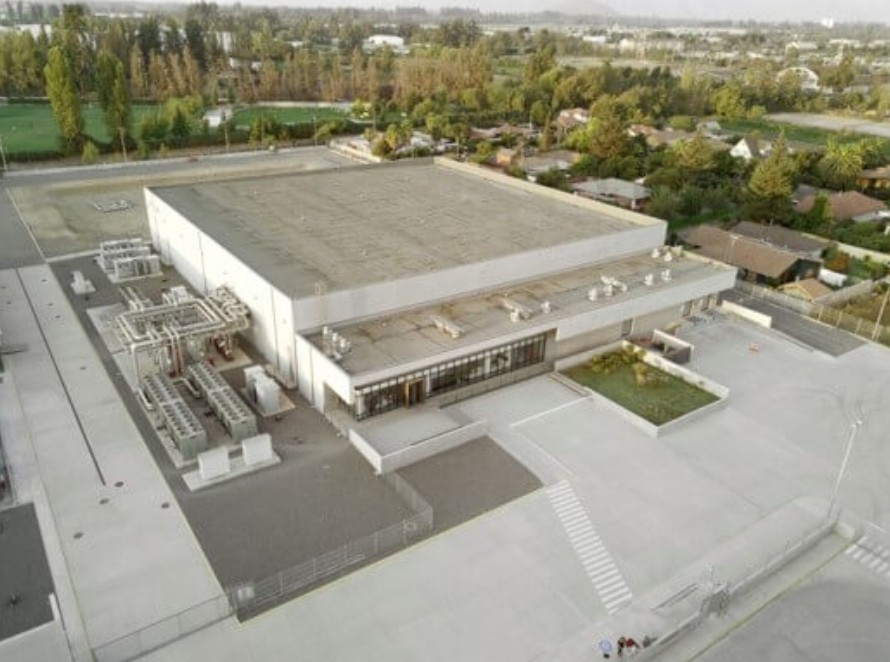
\includegraphics[width=0.7\textwidth]{img/datacenter/chile}	
	\caption{Infraestructura del centro de datos de Telefónica en Chile.}
	\label{img:chile}
\end{figure}

Entre las principales características del centro de datos en Chile tenemos \citep{telefonicachile}:
\begin{itemize}
	\item Construidos sobre 5 000 $m^2$.
	\item Tiene controles biométricos hasta cámaras de seguridad por cada sala y pasillo, y los guardias hacen rondas cada hora.
	\item Tienen la información en diferentes espacios.
	\item La energía llega a un transformador y luego al UPS que que mediante un tablero de distribución que se conecta con una sala blanca.
	
	\item 	Tienen ampolletas de agua presurizadas en todas las salas en caso de incendio.
	2 equipos de climatización para mantener los equipos a una temperatura estable.
	
	\item 	Ingresa aire frío también por un piso falso.
	
	\item 	Sala blanca, con 1000 metros cuadrados para el alojamiento de servidores de 3,25 millones de servidores.
	
	\item 	La sala blanca cumple con los estándares internacionales de seguridad como un pisco falso, conexiones con cables de cobre y fibra óptica ubicados en la parte superior y tienen un monitoreo 24/7 de la energía, humedad y temperatura de la sala.
	
	\item  Tiene una subestación eléctrica encargada de brindar energía a la sala blanca y todas las instalaciones del data center con una potencia de 1,5 KW por metro cuadrado.
	
	\item En caso de un apagón se activa uno de los 3 generadores del grupo electrónico, cada uno tiene una potencia de 2 MW y funciona por más de 60 horas por autonomía.
	
	\item Tienen una planta fría que mantiene la temperatura entre 18 a 27 grados celsius.
	
	\item Tienen un sistema de refrigeración adiabática que mejora el consumo de energía. 
	
	\item 	Disponibilidad del 99.986\% debido a sus 2 fuentes de energía comercial y a un sistema de redundancia electromecánico.
	
	\item Tienen un centro de operaciones donde monitorea la infraestructura crítica de TI, tienen personal capacitado que atiende 24/7 que atienden y gestionan los requerimientos de los clientes.
\end{itemize}
	

	
	
	
\subsubsection{Alcalá de Henares en España}

En la ciudad de Alcalá de Henares (España) esta situado otro centro de datos de Telefónica. En la Figura \ref{img:spania}, mostramos una fota de dicho centro de datos. 

\begin{figure}[H]
	\centering
	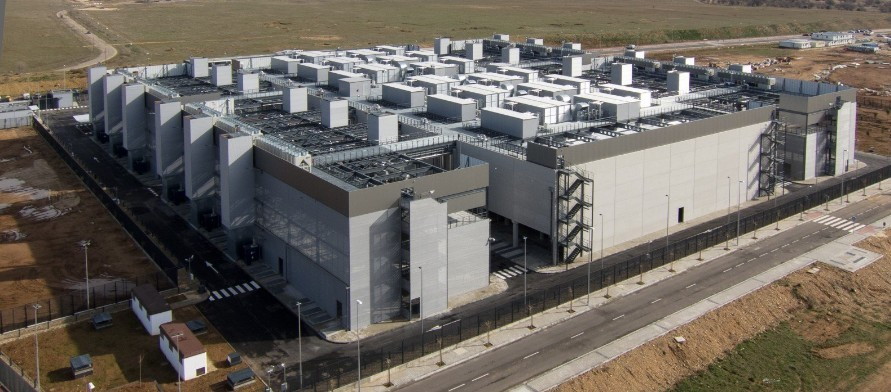
\includegraphics[width=\textwidth]{img/datacenter/espania}	
	\caption{Infraestructura del centro de datos de Telefónica en España.}
	\label{img:spania}
\end{figure}

Entre las principales características del centro de datos en España tenemos \citep{telefonicaespania}:

\begin{itemize}
\item Espacio de TI llega hasta 15 000 $m^2$.
Tiene 7 salas de TI.
\item Cada Sala de TI, tiene 1200 KW de potencia, equivalente a 1,76 KW $m^2$.
\item Tiene doble alimentación eléctrica de 20 MW.
\item Tiene una subestación eléctrica de doble alimentación de 100 MW.
\item Tiene la capacidad de expandirse hasta 23 salas de 682 $m^2$ c/u con una capacidad de potencias de TI de 4 800 kW en cada sala, equivalente a 7 KW por $m^2$.
\item Las medidas de seguridad físicas y virtuales cuentan con un Tier IV en Diseño por el Uptime Institute, lo que significa que cada componente de la instalación, grupo electrógeno, UPS, baterias, fuentes de alimentación, enfriadores, climatizadores de aires, depósitos de agua y diesel, conductos, tuberías,comunicaciones y conectividad, todo es tolerante a fallos.
\item Disponibilidad del 99.995\% por ser Tier IV.
\item Está equipado con subsistemas totalmente redundantes.
\item Corredor de seguridad perimetral con doble verja y portones de acceso, video vigilancia, zonas de seguridad estrictamente compartimentadas, sistema de detección y extinción automática de incendios, todo atendido de forma continua desde un control central de seguridad.
\item La instalación es increíblemente robusta y altamente resistente a fallas y completamente segura.
\item Es ecológica ya que utiliza el Free Cooling direct para climatización y control de temperatura del aire; consistente en utilizar el aire exterior para refrigeración de las salas  de TI.
\item Realiza recuperación de información ante desastres porque realizan copias automática de datos en otros Data Center de otros países, así que pase lo que pase la información estará protegida y disponible.
\end{itemize}

	
	
	
\subsubsection{Ixtlahuaca de Méjico}

En la ciudad de Ixtlahuaca de Méjico esta situado otro centro de datos de Telefónica. En la Figura \ref{img:mexico}, mostramos una fota de dicho centro de datos. 

\begin{figure}[H]
	\centering
	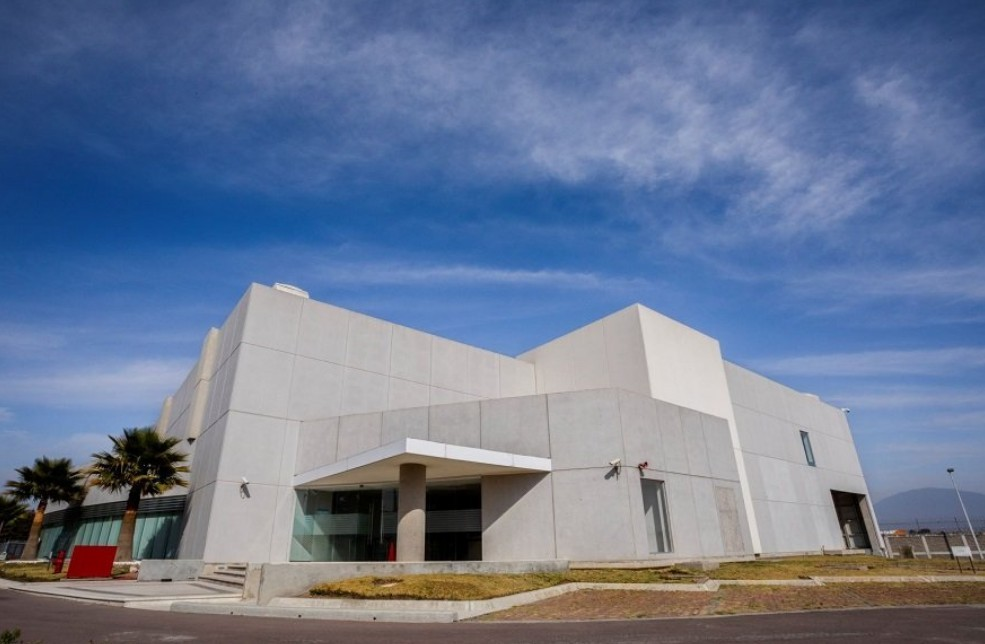
\includegraphics[width=0.7\textwidth]{img/datacenter/mexico}	
	\caption{Infraestructura del centro de datos de Telefónica en Méjico.}
	\label{img:mexico}
\end{figure}

Entre las principales características del centro de datos en Méjico tenemos \citep{telefonicamexico}:

\begin{itemize}
	\item Cumple con lineamientos TIA-942 para un Data Center Tier III.
	\item Tiene más de 18000 $m^2$
	\item Tiene cámaras de 360° de inyección y retorno de aire.
	\item Tiene sistemas de seguridad, monitoreo y soporte 24/7 con profesionales de diversas especialidades.
	\item Disponibilidad de 99.982\%
	\item Ofrece servicios de comunicación unificada, almacenamiento, virtualización, hosting dedicado, housing y otros.
	\item Tiene un sistema ecológico. 
	\item Tienen una capacidad de procesamiento de datos equivalente a alojar 6 000 computadoras portátiles.
	\item Almacenan 152 millones de minutos de llamadas de voz al mes y 240 Terabytes de tráfico de datos por mes.
	\item Tienen varios SOC (Security Operation Center) que monitorean constantemente los Data Center.
	
\end{itemize}
	

\subsubsection{Monterrico en Guatemala}

En la ciudad de Monterrico en Guatemala esta situado otro centro de datos de Telefónica. En la Figura \ref{img:guatemala}, mostramos una fota de dicho centro de datos. 

\begin{figure}[H]
	\centering
	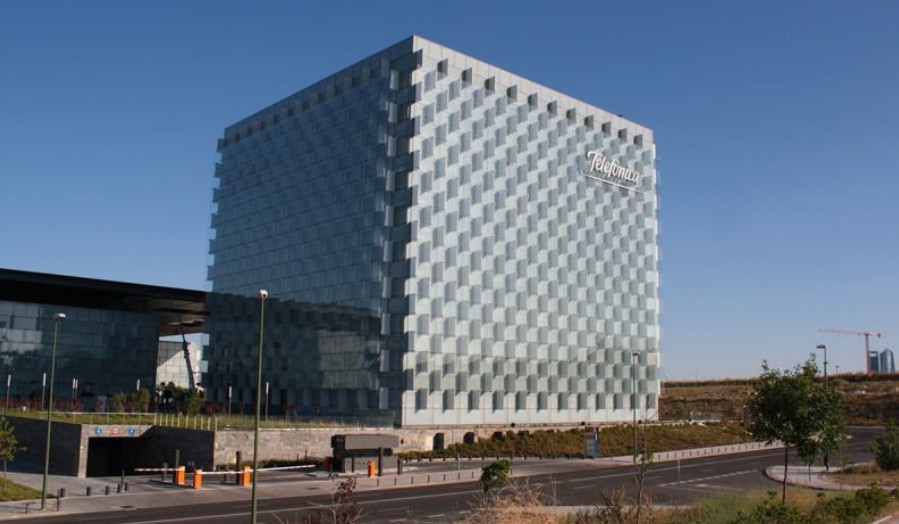
\includegraphics[width=0.7\textwidth]{img/datacenter/guatemala}	
	\caption{Infraestructura del centro de datos de Telefónica en Guatemala.}
	\label{img:guatemala}
\end{figure}

Entre las principales características del centro de datos en Méjico tenemos \citep{telefonicaguatemala}:

\begin{itemize}
	\item El Data Center de Monterrico cuenta además con importantes certificaciones como: Tier III en Diseño por el Uptime Institute, ISO27001 Norma de Seguridad de la Información, ISO 9000 en Calidad en la atención y desarrollo de productos TI, ISO 20000 en Gestión de Servicios TI para outsourcing desktop, PCI Estándar de Seguridad de Datos requerida por el sector financiero y Certificación SAP Hosting Partner Advanced, que permite ofrecer servicios acorde a estándares y buenas prácticas SAP. Los procesos de gestión y operaciones están alineados a buenas prácticas ITIL y PMI.
	\item Esta unidad de negocio cuenta con un clúster propio ubicado en el data center de la compañía en Guatemala, dotado de 19 nodos redundados con capacidad de almacenamiento de 1,3 petabytes.
	
	
\end{itemize}

\section{Conclusiones}

Telefónica es una empresa controversial, pero con vigencia en varios países. Si bien es cierto cuenta varios centros de datos, algunos de ellos han sido vendidos a Asterion, pero Telefónica aún hace uso de ellos. De igual forma, la empresa vendio cuatro centros de datos a cambio del 20\% de Nabiax\\

Adiconalmente Telefónica tiene certificación  Tier III en la mayoria de sus centros de datos e incluso el centro de datos de España cuenta con una certificación Tier IV.  \\

Lamentablemente no hay mucho detalle específico de los centro de datos de Telefónica, pero gracias a información de la misma página de telefónica y sus videos de presentación de sus centro de datos, se ha recolectado información en este documento. \\

	
	

\bibliographystyle{apalike}
%\bibliographystyle{IEEEtranN}
\bibliography{bibliography}

	
	
	
	
\end{document}